\documentclass[11pt]{amsart}


\usepackage{geometry}                % See geometry.pdf to learn the layout options. There are lots.
\geometry{a4paper}                   % ... or a4paper or a5paper or ...
%\geometry{landscape}                % Activate for for rotated page geometry
\usepackage[parfill]{parskip}    % Activate to begin paragraphs with an empty line rather than an indent
\usepackage{enumitem}
\usepackage{graphicx}
\usepackage{amssymb}
\usepackage{amsmath}
\usepackage{cancel}
\usepackage{epstopdf}
\DeclareGraphicsRule{.tif}{png}{.png}{`convert #1 `dirname #1`/`basename #1 .tif`.png}
\usepackage{breqn}
\usepackage{float}

\title{Econ 210C Problem Set \# 2}
\author{Minki Kim}
%\date{}                                           % Activate to display a given date or no date

\begin{document}




\maketitle

\section{Investment and the Housing Market}
\begin{enumerate}[label=(\alph*)]
	\item Explain the model 
\begin{enumerate}
	\item $I = \psi (P)$: Gross investment in housing is an increasing function of the price of houses. This specification implies that housing investment can be interpreted as a supply of new housings. 
	\item $r + \delta = (R + \dot{P})/P$: I assume that $\delta$ denotes the depreciation rate of a house. LHS is opportunity costs of investing into a house: forgone real interest rate and depreciation of the house. RHS is benefits of investing into a house: (real) rental payment and capital gains from the price of house. 
	\item $R = R(H)$: Rental cost $R$ is a decreasing function of available quantity of housing stock. 
	\item $\dot{H} = I - \delta H$: Change in $H$ is the difference between housing investment (new housing) and depreciated housing stock. 
\end{enumerate}
The model is closed: it has 4 endogenous variables ($I,R,P,H$) with 4 equations.

\item Reduce the model into a 2-equation system
\begin{align*}
\dot{H} &= \psi(P) - \delta H \\
r + \delta &= (R(H) + \dot{P}) / P
\end{align*}
Here $R$ is a function, not a variable. 
\item Draw phase diagram. 
*Lines do not have to be linear. 
\begin{figure}[H]
	\centering
	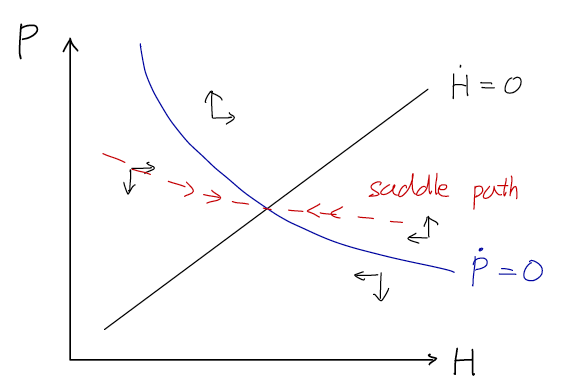
\includegraphics[width=0.65\textwidth]{1c_Minki.png}
	\caption{Phase diagram for the housing market}
\end{figure}
\item Steady state effect of an increase in the real interest rate
$r$ only shows up in the equation for $\dot{P}$. Rewriting the equation: 
\begin{equation*}
\dot{P} + R(H) = P (r + \delta)
\end{equation*}
Given a level of $P$, an increase in $r$ makes RHS larger, requiring $R(H)$ getting larger by the same amount to satisfy $\dot{P} = 0$. Since $R$ is a decreasing function of $H$, it means that $H$ has to decrease. Hence, $\dot{P} = 0$ locus shifts to the left. 

\item Permanent increase in the real interest rate. Suppose the real interest rate changes from $r$ to $r^{*}$, where $r < r^{*}$. Recall that in the initial steady state, $P = \frac{R(H)}{r+\delta}$. At the arrival of the change, $P$ drops to the level $\frac{R(H)}{r^{*} + \delta}$. Cheaper real price of housing assets (or higher opportunity cost of investing in housing) reduces the amount of housing investments. As the housing investment decreases, the quantity of housing stock gradually decreases, until $R(H)$ goes up enough to satisfy $\dot{P}=0$ again.   
\begin{figure}[H]
	\centering
	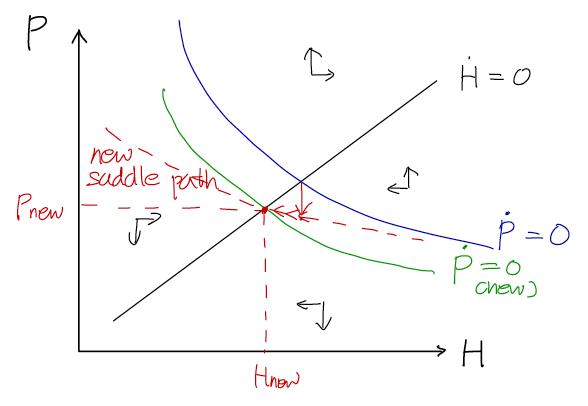
\includegraphics[width=0.65\textwidth]{1e1_Minki.png}
	\caption{Phase diagram for a permanent increase in the real interest rate}
\end{figure}
Below is the impulse responses of each variable in response to the interest rate change. 
\begin{figure}[H]
	\centering
	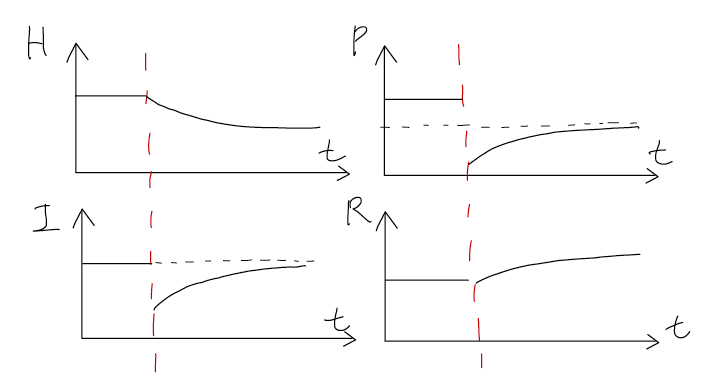
\includegraphics[width=0.7\textwidth]{1e2_Minki.png}
	\caption{Effect of permament increase of $r$ on $H,P,I,R$ }
\end{figure}
\item Temporary increase in the real interest rate 
\item An announced (anticipated) permanent increase in the real interest rate
\item Static expectation
\item Use of this model to analyze the housing crisis
\end{enumerate}

\section{Discount Factor Shock}
Time-varying discount factor is being incorporated in the model through the Euler equation. Below is the model developed in the class with time-varying discount factor. 
\begin{align*}
\lambda_t &= \frac{1}{C_t} \\
\frac{C_{t+1}}{C_t} &=  \mathbb{E}_t \beta_{t+1} (1+ R_{t+1})\\
W_t &= (1-\alpha) Z_t \left( \frac{K_{t-1}}{L_t} \right)^\alpha \\
R_t + \delta & = \alpha Z_t \left( \frac{K_{t-1}}{L_t} \right)^{\alpha-1} \\
L_t^{\frac{1}{\eta}} C_t &= W_t \\
C_t + I_t + G_t &= Z_t L_t \left(\frac{K_{t-1}}{L_t} \right)^\alpha \\
K_t &= (1-\delta) K_{t-1} + I_t
\end{align*}

The model has seven endogenous variables ($\lambda_t, K_t, W_t, C_t, L_t, R_t, I_t$ ) and three exogenous variables ($\beta_t, Z_t, G_t)$. We can also reduce the model into a 2-equation system. A log-linearized version of the system is as follows:

\begin{align*}
\Delta \check{K_t} &= \frac{\bar{Y}}{\bar{K}} \left( 1 + \frac{1-\alpha}{\alpha + 1/\eta} \right) \check{Z_t} + \left( \frac{\alpha (1-\alpha )}{\alpha + 1/\eta}  \frac{\bar{Y_t}}{\bar{K_t}}  + \alpha \frac{\bar{Y}}{\bar{K}} - \delta  \right) \check{K_{t-1}}  \\
&+ \left( \frac{\bar{C}}{\bar{K}} + \frac{\bar{Y}}{\bar{K}} \frac{(1-\alpha)}{\alpha + 1/\eta}\right) \check{\lambda_t} - \frac{\bar{G}}{\bar{K}}\check{G_t} \\
\Delta \check{\lambda_{t+1}}  &=  - \check{\beta_{t+1}} - \frac{\alpha \frac{\bar{Y}}{\bar{K}}}{\alpha \frac{\bar{Y}}{\bar{K}} + 1 - \delta} \left[   \left( 1 + \frac{1-\alpha}{\alpha + 1/\eta} \right) \check{Z_{t+1}} + (1-\alpha) \left( \frac{\alpha}{1/\eta + \alpha} -1 \right) \check{K_t} + \frac{1-\alpha}{1/\eta + \alpha} \check{\lambda_{t+1}}  \right]
\end{align*}

By setting $\Delta \lambda_t = 0$, we have the locus of points where the marginal utility of wealth is not changing.
\paragraph{\bf Locus $\Delta \lambda_t = 0$} 
\begin{equation*}
\check{\lambda_{t+1}} = -  \frac{1/\eta + \alpha}{1-\alpha} \left[  \left( \frac{\alpha \frac{\bar{Y}}{\bar{K}}}{\alpha \frac{\bar{Y}}{\bar{K}} + 1 - \delta} \right)^{-1} \check{\beta_{t+1}} +  \left( 1 + \frac{1-\alpha}{\alpha + 1/\eta} \right) \check{Z_{t+1}} + (1-\alpha) \left( \frac{\alpha}{1/\eta + \alpha} -1 \right) \check{K_t} \right] 
\end{equation*}

Since $\check{\beta_t}$ does not change the slope of the $\Delta \lambda_t$ locus, the phase diagram for this economy is similar to the one we drew in class. 

\paragraph{ \bf Permanant discount factor shocks}
The increase in the discount factor means that agents become more patient - they value future utility relatively more than before. This means that they want to consume less in the present period and more in the future, relative to those people with lower discount rate. 
\begin{figure}[H]
	\centering
	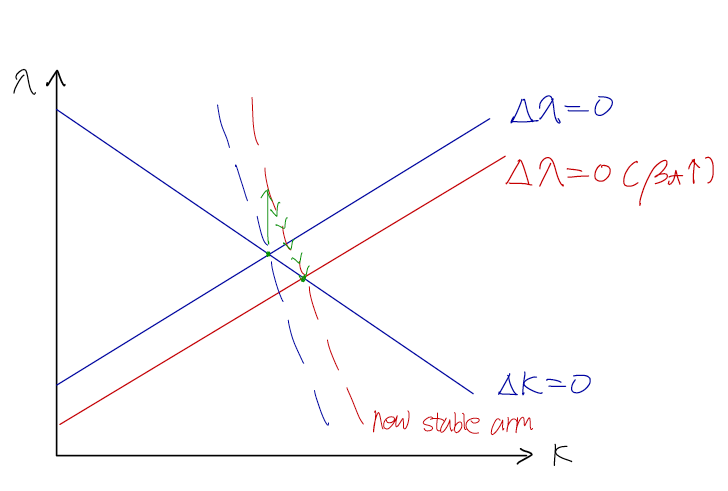
\includegraphics[width=0.7\textwidth]{2_1_Minki.png}
	\caption{Response to permanent discount factor shock}
\end{figure}
In response to the shock, marginal utility jumps up to the new stable arm, inducing higher labor supply and investment along with lower consumption. Marginal utility and investments gradually decrease as the economy approaches to the new steady state, chracterized by a higher capital stock and steady state consumption level. With more capital stock being accumulated, labor demand also increases, building up higher aggregate labor as well as output. Steady state wage is higher than the wage before the shock, since steady state interest rate is lowered ($\because R = \frac{1}{\beta}$). This implies that labor demand reacts more aggresively relative to labor supply. Transition paths for each variable are summarized in the table below. 
\begin{table}[H]
	\centering
	\begin{tabular}{cccc}
		\hline \hline 
		& Impact  & Transition            & Steady State \\
		& $t=t_0$ & $t \in (t_0, \infty)$ & $t = \infty$ \\
		\hline 
		$\lambda$ &   $\uparrow$      &   $\downarrow$   &   $\downarrow$     \\
		$K$           &   0                      &   $\uparrow$       &    $\uparrow$    \\
		$C$           &  $\downarrow$   &   $\uparrow$       &     $\uparrow$       \\
		$L$           &   $\uparrow$       &    $\uparrow$       &  $\uparrow$            \\
		$Y$           &   $\uparrow$       &     $\uparrow$      &   $\uparrow$           \\
		$I$            &   $\uparrow$       &  $\downarrow$   & $\uparrow$              \\
		$W$          &   $\downarrow$  &   $\uparrow$       &      $\uparrow$        \\
		$R$           &   $\uparrow$       &    $\downarrow$ &     $\downarrow$        \\
		\hline
	\end{tabular}
	\caption{Response to a permanent discount factor shock}
\end{table}
\paragraph{\bf Transitory discount factor shocks}
In response to a transitory discount factor shock, marginal utility jumps up just to make sure to land on the initial stable arm when the shock disappears at $t= t_1$. 
\begin{figure}[H]
	\centering
	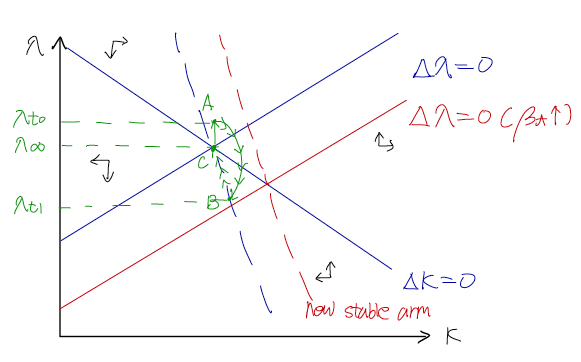
\includegraphics[width=0.7\textwidth]{2_2_Minki.png}
	\caption{Response to transitory discount factor shock}
\end{figure}

\begin{figure}[H]
	\centering
	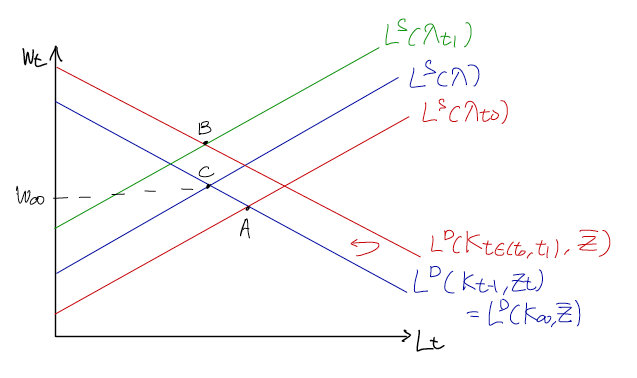
\includegraphics[width=0.7\textwidth]{2_3_Minki.png}
	\caption{Labor market response to transitory discount factor shock}
\end{figure}
At the time of shock $(t_0)$, $\lambda$ jumps up, inducing higher labor supply and lower consumption. Higher output with less consumption means higher investment, followed by a larger stock of capital. Higher labor supply induces lower real wage, and with no change in productivity it means that higher real interest rate (FPPF argument). 

In constrast to a permanent shock, the economy accumulates more capital only to support temporarily higher consumption level while the shock persists. In the course of the period that the shock is effective, households gradually increase their consumption and decrease labor supply, eating up the capital they accumulated earlier. This is demonstrated in the above labor supply curve. Since labor demand also increases due to the higher capital stock, the effect of a transitory discount shock on aggregate labor (hence output) largely depends on the elasticity of labor supply and labor demand.  

After period $t_1$, the economy follows the initial stable arm and returns to the initial steady state. Consumption goes back to its initial level, along with higher labor supply to support it. Since we can't sign aggregarte labor, we can't use production function to sign output. However, Using $Y = C+ I$ we can back out the sign of $Y$. Transition dynamics are summarized in the table below.   
\begin{table}[H]
	\centering
	\begin{tabular}{cccccc}
		\hline \hline 
		& Impact  & Transition I          & Inflection & Transition II & Steady State  \\
		& $t=t_0$ & $t \in (t_0, t_1)$ & $t = t_1$ & $t \in (t_1, \infty)$ & $t = \infty$ \\
		\hline 
		$\lambda$ &  $\uparrow$    &    $\downarrow$     &    0     & $\uparrow$ &0     \\
		$K$           &      0                &    $\uparrow \rightarrow \downarrow$  &   0      & $\downarrow$ &    0\\
		$C$          & $\downarrow$ &   $\uparrow$      &   0      & $\downarrow$ &    0\\
		$L$          &   $\uparrow$    &   ?      & 0     &  ? &      0\\
		$Y$          &    $\uparrow$   &    ?    &    0    &  $\downarrow$  &      0\\
		$I$           &   $\uparrow$    &  $\uparrow \rightarrow \downarrow$  & 0 & $\downarrow$  &    0\\
		$W$         & $\downarrow$ &    $\uparrow$     &    0     & $\downarrow$ &  0   \\
		$R$          &  $\uparrow$    &     $\downarrow$     &    0     & $\uparrow$  &  0 \\
		\hline
	\end{tabular}
	\caption{Response to a transitory discount factor shock}
\end{table}


\section{(Noise) News Shock}
\section{Labor Supply}
\begin{enumerate}[label=(\alph*)]
	\item Since the path of the wage rate $w_t$ is known at $t=0$, there is no uncertainty in the economy. To prepare for the days when $w_t$ level is not high enough to compensate the consumption level $C$ she would like to spend every period, she has to save some fraction of her income. Let the saving in period $t$ be $S_t$. Her intertemporal and lifetime budget constraints are written as follows: 
	\begin{align*}
	C + S_t &= w_t N_t + S_{t-1} \\
	\sum_{t=0}^{T} w_t N_t & = C \times T
	\end{align*} Now set up a Lagrangian: 
	\begin{equation*}
	\mathcal{L} = \sum_{t=0}^{T}  \left[ \ln (1+ N_t) + \lambda_t \left(C + S_t - w_t N_t - S_{t-1} \right) \right] + \psi \sum_{t=0}^{T} \left( w_t N_t - C \cdot T\right)  
	\end{equation*}
    Let's not focus on the additional equations concerned with the first and last periods. First order conditions for $S_t$ and $N_t$ are: 
    \begin{align*}
    \lambda_t &= \lambda_{t+1} \\
    \frac{1}{1+N_t} + \psi w_t &= \lambda_t w_t 
    \end{align*}
    Combining the above two equations gives us the Euler equation: 
    \begin{equation*}
    w_t (1+ N_t) = w_{t+1} (1+N_{t+1})
    \end{equation*}
    \item Rearrage the Euler equation: 
    \begin{equation*}
    \frac{w_{t+1}}{w_t} = \frac{1+N_t}{1+ N_{t+1}} = \frac{\text{Marginal disutility of labor in period $t+1$ } (MU_{t+1}) }{\text{Marginal disutility of labor in period $t$ } (MU_t) }
    \end{equation*}
    If wage goes up in current period, either $MU_t$ goes up or $MU_{t+1}$ goes down, which means the individual either works more in this period to take advantage of the higher wage, or work less in the next period using up increased savings accumulated in period $t$. 
    
    \item The Euler equation implies that current labor supply depends on not only current wage level, but also future levels of wage and lagor supply. 
    \item If the wage level goes up \textit{permanently}, the Euler equation and the fact the agent only want to consume fixed $C$ every period tells us the agent will work less for all periods. In other words, positive wealth effect induces less working hours. 
    \item Same logic as in $(b)$ applies. For an anticipated wage increase, the agent either decide to work less in this period and take advantage of higher wage in the future, or work more in the periods when wage is higher and work less after the shock dissipates (If the wage raise is temporary).
    \item Take log on the Euler equation and rearrange:
    \begin{align*}
    \log \frac{w_{t+1}}{w_t} &= \log \frac{1+N_{t+1}}{1+ N_t} \\
    d (log w_{t+1}) &= -d (log (1+N_{t+1}))
    \end{align*}
    Therefore this example implies that labor supply elasticity is always one. 
\end{enumerate}
\section{Impulse Responses}
\begin{enumerate}[label = (\alph*)]
	\item Simulated values of output, consumption, investment and capital are shown in the below graph. 
	\begin{figure}[H]
		\centering
		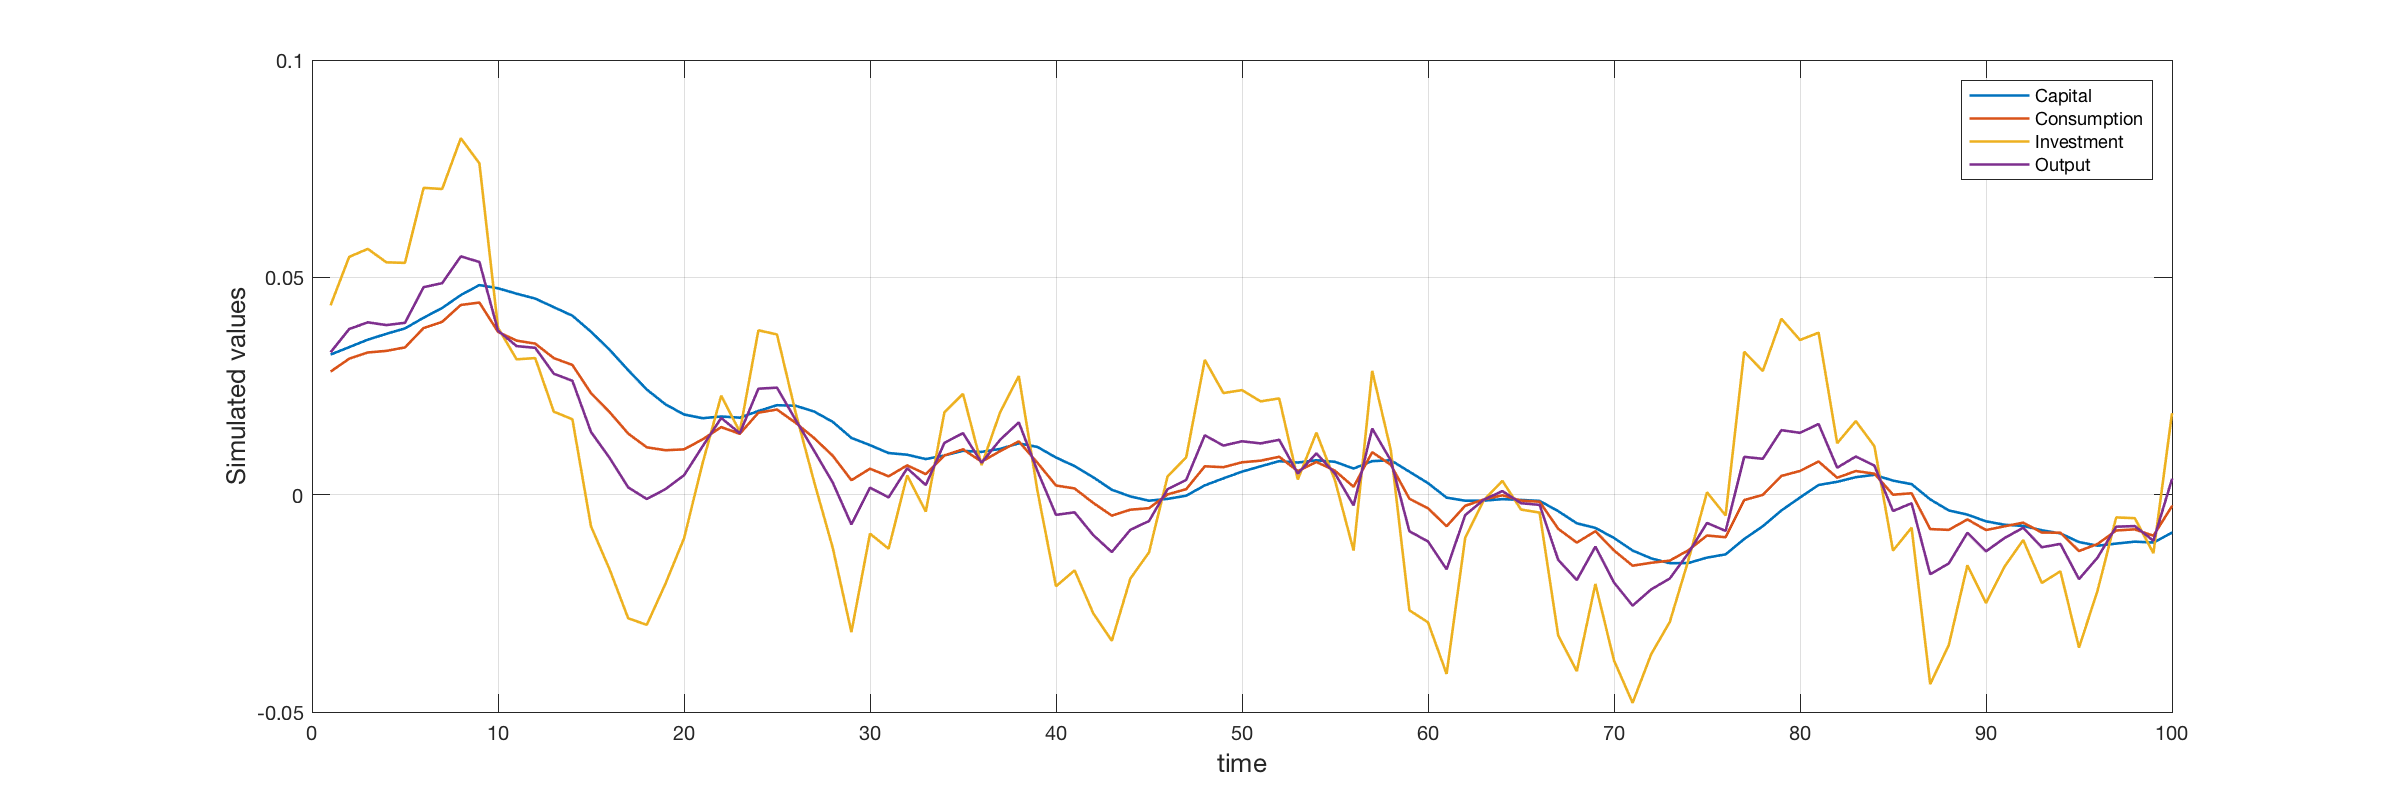
\includegraphics[width=1\textwidth]{5a_Minki.png}
		\caption{Simulated business cycles}
	\end{figure}
    Volatilities (sample standard deviations) of key aggregate variables are compared to the estimates from Stock and Watson paper. Below table summarizes the result. 
    \begin{table}[H]
    	\centering
    	\begin{tabular}{ccc}
    		\hline \hline 
    		 \bf Variable  & \bf Simulation StDev           & \bf Stock and Watson \\
    		\hline 
    	    Output                &  2.59       &   1.66      \\
    		Consumption      &   2.19      &   1.26         \\
    	    Investment         &   3.93      &    4.97       \\
    		\hline
    	\end{tabular}
    	\caption{Comparison of volatilities to Stock and Watson }
    \end{table}
    Simulated investments are more volatile than consumption and output, but less than the estimate from the actual data. Consumption is less volatile than output, which is consistent with the data. 
    
    \item Since labor supply is inelastic, the deviation of wage is equal to the deviation of output in a log-linearized model. Below is the impulse response of consumption, output, investment, and technology to a unit shock in technology. 
    
    I assume that $\varepsilon_t$ was zero before period $t$, becomes 0.01 at period $t$, and returns to zero afterward. 
    \begin{figure}[H]
    	\centering
    	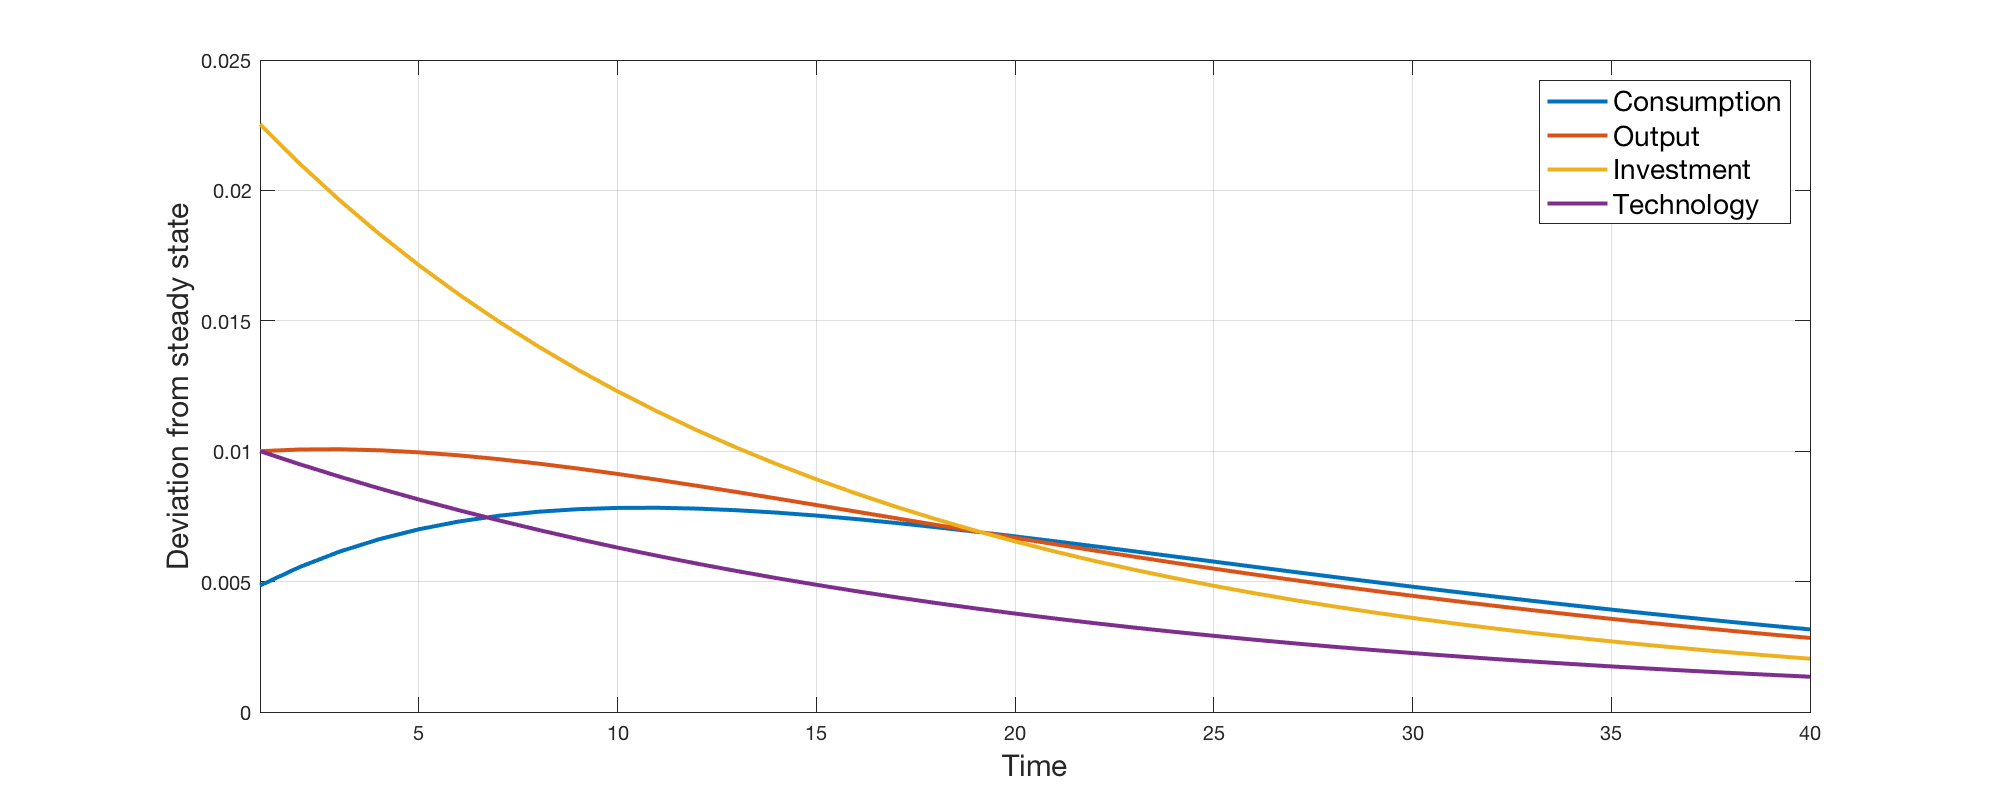
\includegraphics[width=1\textwidth]{5b_Minki.png}
    	\caption{Impulse response}
    \end{figure}
    
    
    \item 
\end{enumerate}
\section{Impulse Responses (2)}



\end{document}
